\section{System Correctness}
\label{sec:evaluation:system-correctness}

In order to determine the system correctness, 
given the inaccuracy of the indoor positioning described in \Cref{sec:estimoteprecision}, 
we created a simulation of the system.

The purpose of the simulation is to calculate how often the user \emph{actually} points at the intended device, 
given some inaccuracy of the indoor positioning.

The system is based on multiple \textit{setups}. 
Each setup consists of the following parameters:
\begin{itemize}
\item \texttt{roomSize}: The size of some room.
\item \texttt{position}: A position of the user in the room.
\item \texttt{devices}: The devices available in the room.
\item \texttt{focusedDevice}: The device the user must point at.
\item \texttt{offset}: An offset applied to the users position.
\end{itemize}

For each setup, the simulation calculates the orientation the user must have in order to point at \texttt{focusedDevice}. 
The simulation then performs \num{100} tests for each setup. 
For each of those tests, 
the user's position is offsetted both horizontally and vertically, 
by a total amount of \texttt{offset}. 
The horizontal offset, \ie the offset for $x$, 
is chosen as a random number between $-\var{offset}$ and $\var{offset}$. 
The vertical offset, \ie the offset for $y$, 
is then calculated as $y = \sqrt{\var{offset}^2 - x^2}$. 
We then ensure that $x \geq 0 \wedge x \leq \var{roomSize.width} \wedge y \geq 0 \wedge y \leq \var{roomSize.height}$.

One iteration of the test consists of multiple setups, 
with different values for \texttt{position} and \texttt{focusedDevice}. 
We had \num{3} setups for each device in the system. 
\num{6} devices were included resulting in a total of \num{18} setups.

For each of the \num{18} setups we performed \num{100} tests with different offsets of the user. 
In each of the \num{100} tests, 
we found the set of devices the user points at given his position, 
his orientation and the set of \num{6} devices. 
If the \texttt{focusedDevice} is still in the set of devices the user points at, 
\ie the user points at the intended device,
the test is considered to be accepted. 

The result of performing the \num{1800} tests, 
is a percentage of how often the \texttt{focusedDevice} was in the set of visible devices. 
For example, a test result of \perc{24}, 
indicates that \perc{24} of the time, 
the user still pointed at the desired device, 
even though his location was offset, 
as it would be if we got the position from the Estimote Indoor SDK.

Since there are random numbers in the system, 
we may get slightly different results when performing a test with the exact same input values. 
Therefore we perform the \num{1800} tests \num{10} times each, 
and take the average correctness rate.

This was performed \num{7} times with different offsets, 
in order to see the influence of \texttt{offset},
\ie the influence of the inaccuracy of Estimote.

To sum up:
\begin{enumerate}
\item We tested a number of setups. In our case this is \num{18}, \num{3} for each of the \num{6} devices in the system.
\item \num{100} tests for each of the setups. Each test randomly offsets the user position horizontally and vertically, resulting in a total offset of \texttt{offset}.
\item The set of \num{18} setups is then tested \num{10} times in order to calculate an average accuracy. This results in \num{18000} small tests where the users position is offsetted.
\item This is then done \num{7} times with different values of \texttt{offset}.
\end{enumerate}

\subsection{Configuration}

\Cref{tbl:evaluation:system-correctness:devices} shows the six devices used in the simulation of the system.

\begin{table}[!hbt]
\centering
\caption{Devices used in the simulation.}
\label{tbl:evaluation:system-correctness:devices}
\begin{tabular}{c|c}
	ID &  Coordinate   \\ \hline
	1  & $(6.5, 3.4)$  \\
	2  & $(3.5 , 3.4)$ \\
	3  & $(4.0 , 1.8)$ \\
	4  & $(2.5 , 1.8)$ \\
	5  & $(0.5 , 0.5)$ \\
	6  & $(2.5 , 3.2)$
\end{tabular}
\end{table}

\Cref{lst:evaluation:system-correctness:setups} shows the \num{18} setups tested. 
The set of setups was tested with the offsets shown in \Cref{lst:evaluation:system-correctness:results}, 
along with the achieved accuracy, 
when applying the offset to the users position.

The size of the room used in the setups, 
matches a real world living room in a \SI{80}{\square\meter} apartment. 
\num{6} devices are used, 
as we found it reasonable in a living room of that size.

The positions used are arbitrary, 
and less important when we calculate the orientation, 
based on the users position and the position of the focused device.

\begin{table}[!hbt]
\centering
\begin{tabular}{c|ccc}
	ID &   Position    & Focused device ID & Room size in meter \\ \hline
	1  & $(2.0 , 2.0)$ &         1         & $6.9 \times 5.37$  \\
	2  & $(3.4 , 4.9)$ &         1         & $6.9 \times 5.37$  \\
	3  & $(1.1 , 3.6)$ &         1         & $6.9 \times 5.37$  \\
	4  & $(0.5 , 0.5)$ &         2         & $6.9 \times 5.37$  \\
	5  & $(1.1 , 3.3)$ &         2         & $6.9 \times 5.37$  \\
	6  & $(5.5 , 5.2)$ &         3         & $6.9 \times 5.37$  \\
	7  & $(3.0 , 2.9)$ &         3         & $6.9 \times 5.37$  \\
	8  & $(1.0 , 2.0)$ &         3         & $6.9 \times 5.37$  \\
	9  & $(2.5 , 2.3)$ &         3         & $6.9 \times 5.37$  \\
	10 & $(4.4 , 3.4)$ &         4         & $6.9 \times 5.37$  \\
	11 & $(6.0 , 1.2)$ &         4         & $6.9 \times 5.37$  \\
	12 & $(5.8 , 2.7)$ &         4         & $6.9 \times 5.37$  \\
	13 & $(4.6 , 1.4)$ &         5         & $6.9 \times 5.37$  \\
	14 & $(2.3 , 5.2)$ &         5         & $6.9 \times 5.37$  \\
	15 & $(0.3 , 0.1)$ &         5         & $6.9 \times 5.37$  \\
	16 & $(6.2 , 4.4)$ &         6         & $6.9 \times 5.37$  \\
	17 & $(5.1 , 2.7)$ &         6         & $6.9 \times 5.37$  \\
	18 & $(3.2 , 5.1)$ &         6         & $6.9 \times 5.37$
\end{tabular}
\caption{Setups used in the simulation. Device IDs references \Cref{tbl:evaluation:system-correctness:devices}.}
\label{lst:evaluation:system-correctness:setups}
\end{table}

During all tests a visibility angle of \num{30} degrees was used, 
\ie \num{15} degrees on each side of the users orientation, 
as described in \Cref{sec:analysis:orientation}.

\Cref{fig:evaluation:system-correctness:simulation} illustrates the simulation. 
In this case the user desires to control Device 1 (the rightmost device). 
The figure shows three situations in the simulation. 
\Cref{fig:evaluation:system-correctness:simulation:initial} shows the initial situation, 
in which the user faces the device directly. 
This situation is not considered when calculating the resulting accuracy, 
as this situation always takes place when the orientation of the user is calculated. 
The \emph{accepted} situation is shown in \Cref{fig:evaluation:system-correctness:simulation:accepted}. 
Even though the user's location is offsetted, 
Device 1 is still in his line of sight. 
This is not the case in \Cref{fig:evaluation:system-correctness:simulation:failure}, 
where the offset causes Device 1 to no longer be in the user's line of sight.

Please note that the line of sight in \Cref{fig:evaluation:system-correctness:simulation} is for \emph{illustration purposes only}. 
In reality the line of sight is a triangle of \num{30} degrees, 
from the user pointing in the users orientation.

\begin{figure}[!htb]%
    \centering
    \subbottom[Initial position of the user. The user focuses directly on Device 1 (the rightmost device).]{\label{fig:evaluation:system-correctness:simulation:initial}
        \frame{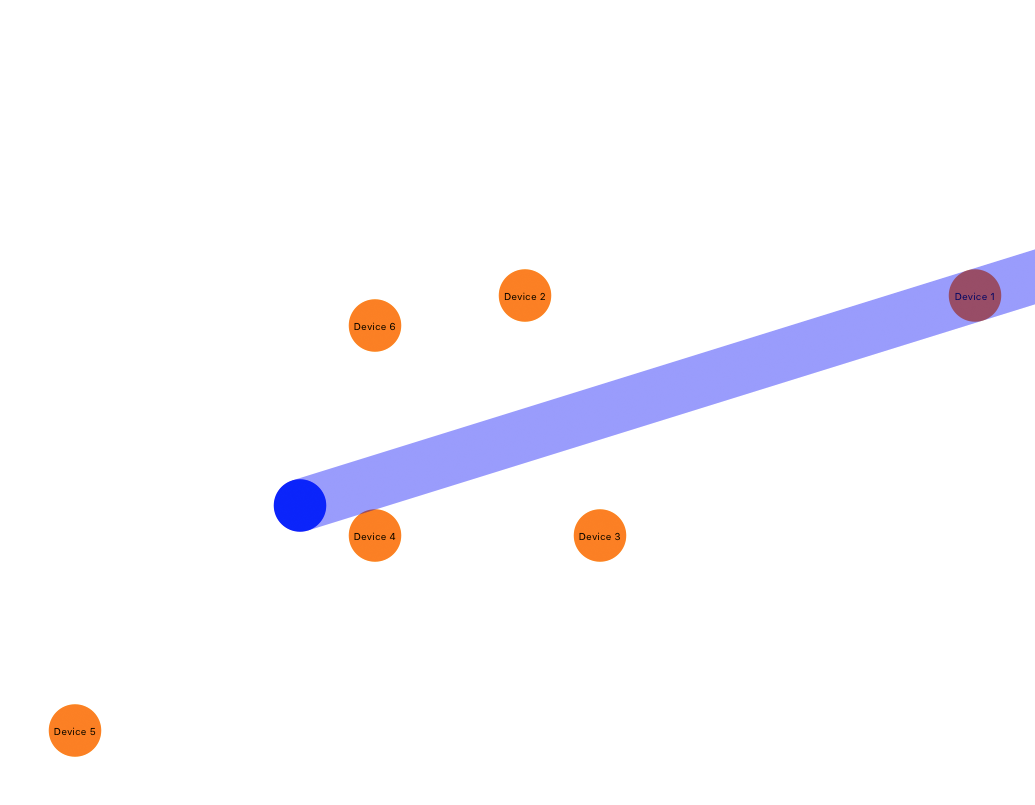
\includegraphics[width=0.3\textwidth]{images/system-correctness-initial}}
    }
    \subbottom[Accepted position of the user. Even though the user's location is offsetted, Device 1 is still in his line of sight.]{\label{fig:evaluation:system-correctness:simulation:accepted}
        \frame{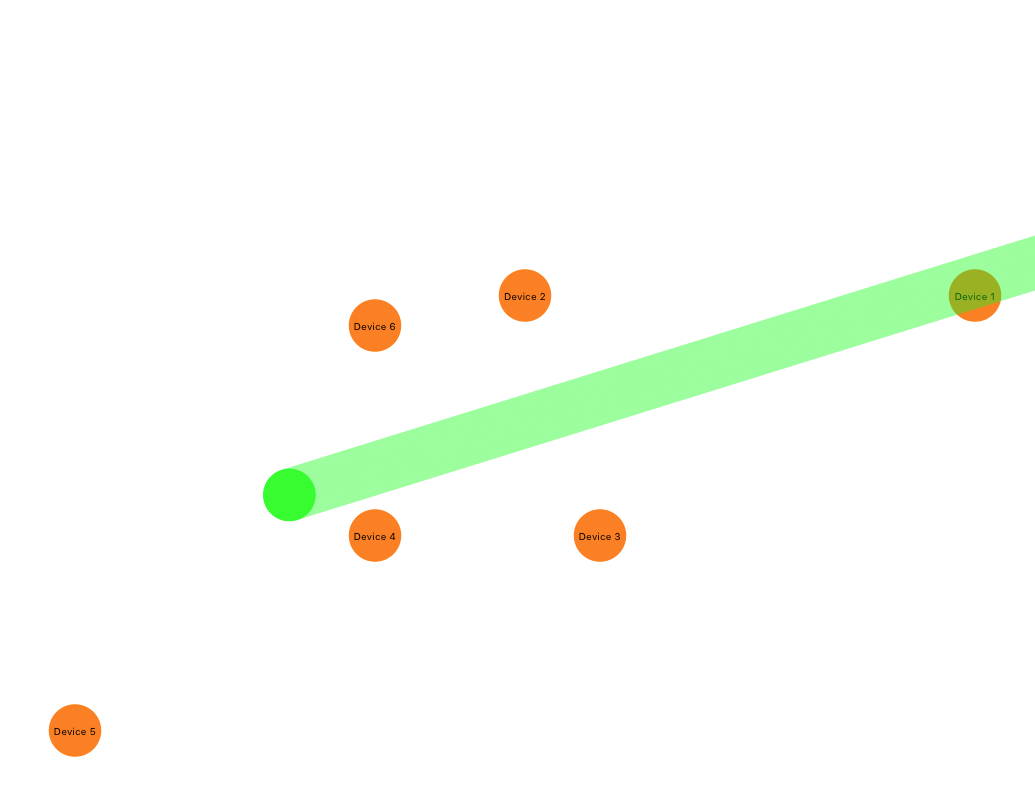
\includegraphics[width=0.3\textwidth]{images/system-correctness-accepted}}
    }
    \subbottom[Rejected position of the user. Due to the offset, Device 1 is no longer in the users line of sight.]{\label{fig:evaluation:system-correctness:simulation:failure}
        \frame{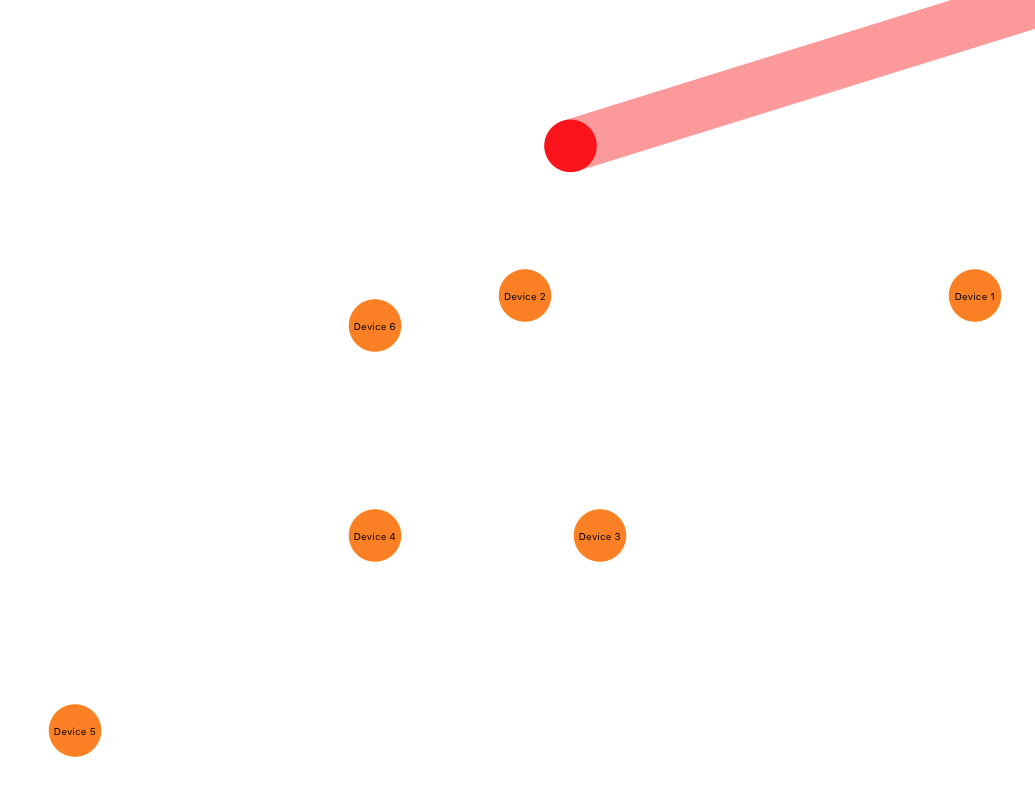
\includegraphics[width=0.3\textwidth]{images/system-correctness-failure}}
    }
    \caption{Illustrations of the simulation. Device 1 is the desired device to be focused.}
    \label{fig:evaluation:system-correctness:simulation}
\end{figure}

\subsection{Results}

\Cref{lst:evaluation:system-correctness:results} shows the results of the simulation. 
We tested the system with offsets from \SIrange{0}{2.92}{\meter} with a \SI{0.5}{\meter} interval. 
We test up to \SI{2.92}{\meter}, 
as this is the average accuracy we measured when testing the precision of Estimote, 
as described in \Cref{sec:estimoteprecision}.

\begin{table}[!htb]
	\centering
	\begin{tabular}{rc}
		           Offset & Percentage of correct points \\ \hline
		   \SI{0}{\meter} &        \perc{100.00}         \\
		 \SI{0.5}{\meter} &         \perc{88.93}         \\
		   \SI{1}{\meter} &         \perc{56.67}         \\
		 \SI{1.5}{\meter} &         \perc{23.54}         \\
		   \SI{2}{\meter} &         \perc{12.56}         \\
		 \SI{2.5}{\meter} &         \perc{6.89}          \\
		\SI{2.92}{\meter} &         \perc{4.29}
	\end{tabular}
	\caption{Results of the seven tests performed. The ``Offset'' column shows the total offset applied to the users position, and the ``Accuracy'' column shows the number of tests, that resulted in the desired device being in the line of sight. The percentage has been rounded to two decimals.}
	\label{lst:evaluation:system-correctness:results}
\end{table}

\begin{figure}[!htb]
    \centering
    \begin{tikzpicture}
  \begin{axis}[
%      ybar,
%      bar width=2pt,
      xlabel = Offset in meters,
      ylabel = Accuracy in percent,
      xtick=data,
      width=0.95\textwidth,
      height = 6cm,
      yticklabel style={align=right,inner sep=0pt,xshift=-0.3em},
      enlargelimits = false,
      ymax = 100,
      grid=major,
      try min ticks=10]]
    \addplot table[x=offset, y=accuracy] {data/system-correctness/results.csv};   
  \end{axis}
\end{tikzpicture}
    \caption{Accuracy of the system for each of the offsets in \Cref{lst:evaluation:system-correctness:results}.}
    \label{fig:evaluation:system-correctness:results}
\end{figure}

Based on the results presented in \Cref{lst:evaluation:system-correctness:results} and illustrated by \Cref{fig:evaluation:system-correctness:results}, 
we can conclude that the system is \emph{not} sufficiently accurate. 
With a mean error of \SI{2.92}{\meter}, 
the system will only point at the desired device \perc{4.29} of the time. 
In order to achieve the desired accuracy of \perc{80} described in the requirements section (\Cref{sec:requirements-specification}), 
we must reduce the offset to less than \SI{\sim 0.6}{\meter}.

Inaccuracy in the orientation of the user, 
which may the result of an inaccurate magnetometer, 
was not simulated in this test. 
From use throughout the project, 
we generally found the magnetometer to be reliable within a few ($\sim 5$) degrees. 
Any inaccuracy in the measurements provided by the magnetometer, 
could be compensated by a wider visibility angle.

%%% Local Variables:
%%% mode: latex
%%% TeX-master: "../../master"
%%% End:
